\begin{figure*}[hbtp]
  \centering
  \subfigure[Runtime in seconds (logarithmic scale) for link prediction using various similarity measures, with IHub approach]{
    \label{fig:pruned1--runtime}
    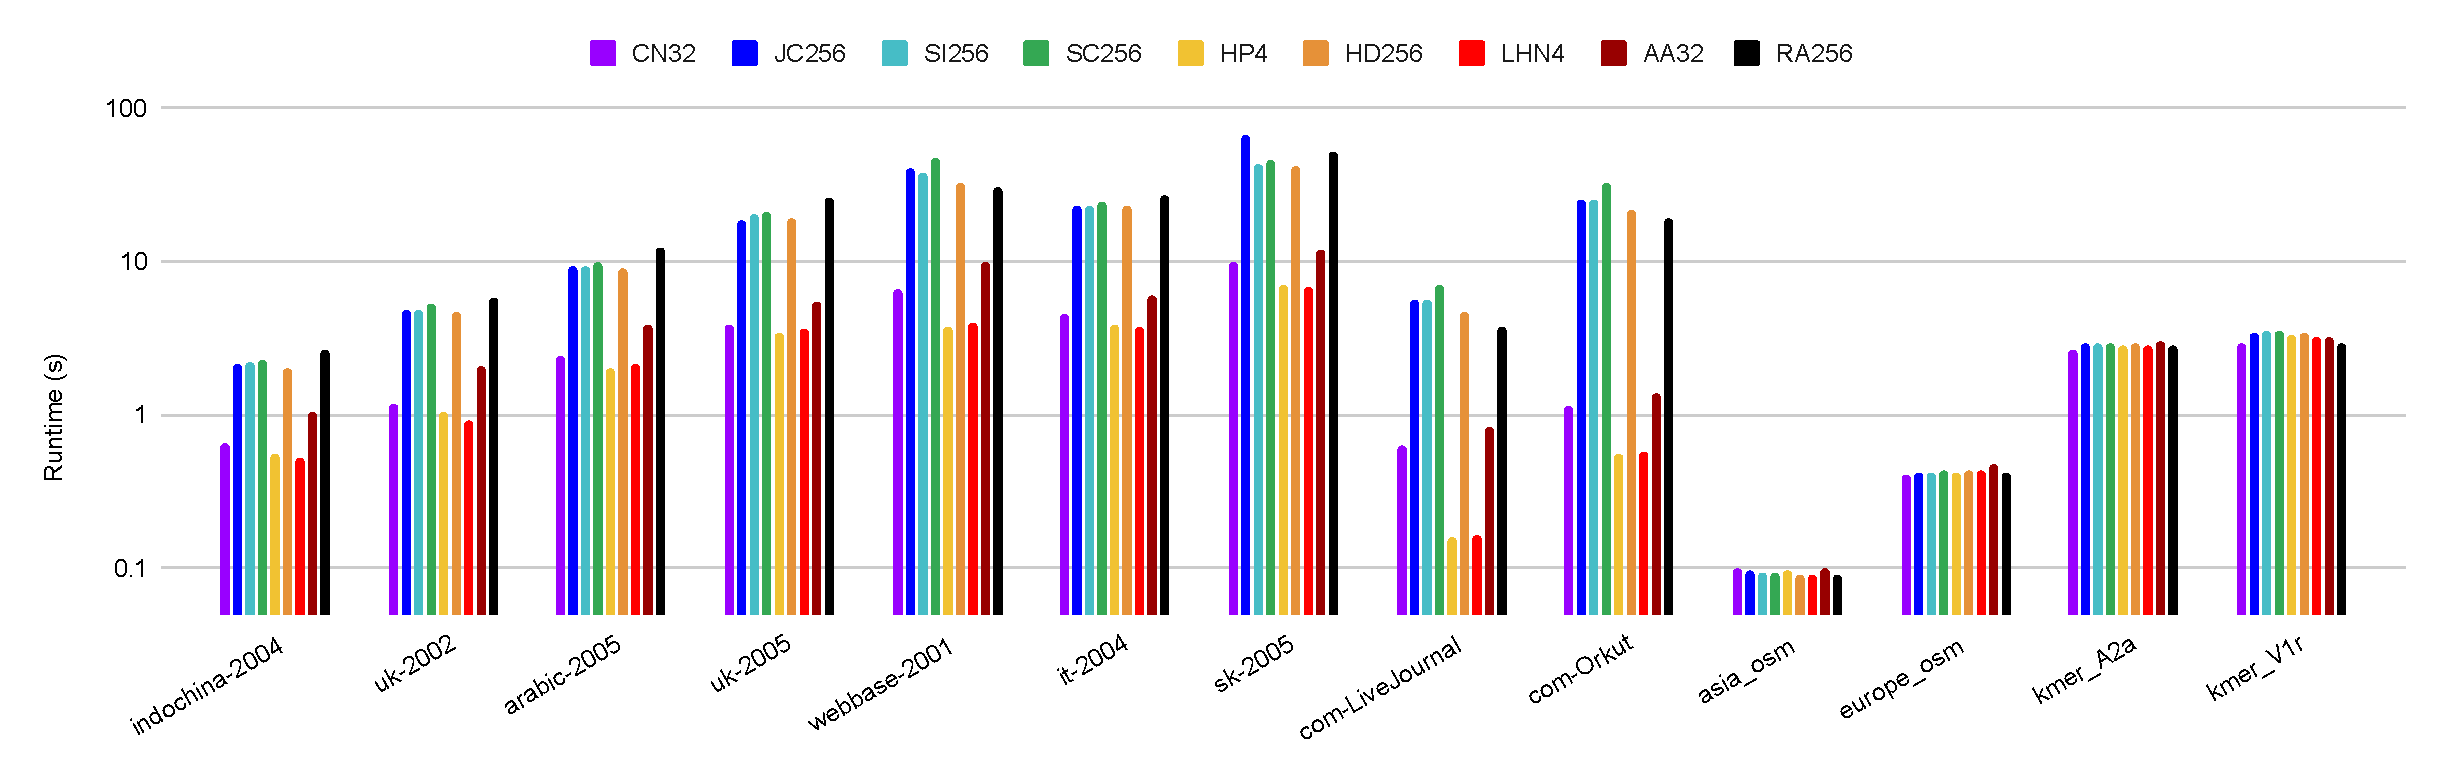
\includegraphics[width=0.98\linewidth]{out/pruned1-runtime.pdf}
  }
  \subfigure[Precision of predicted links, in percentage (logarithmic scale), of the best neighborhood-based link prediction method]{
    \label{fig:pruned1--f1score}
    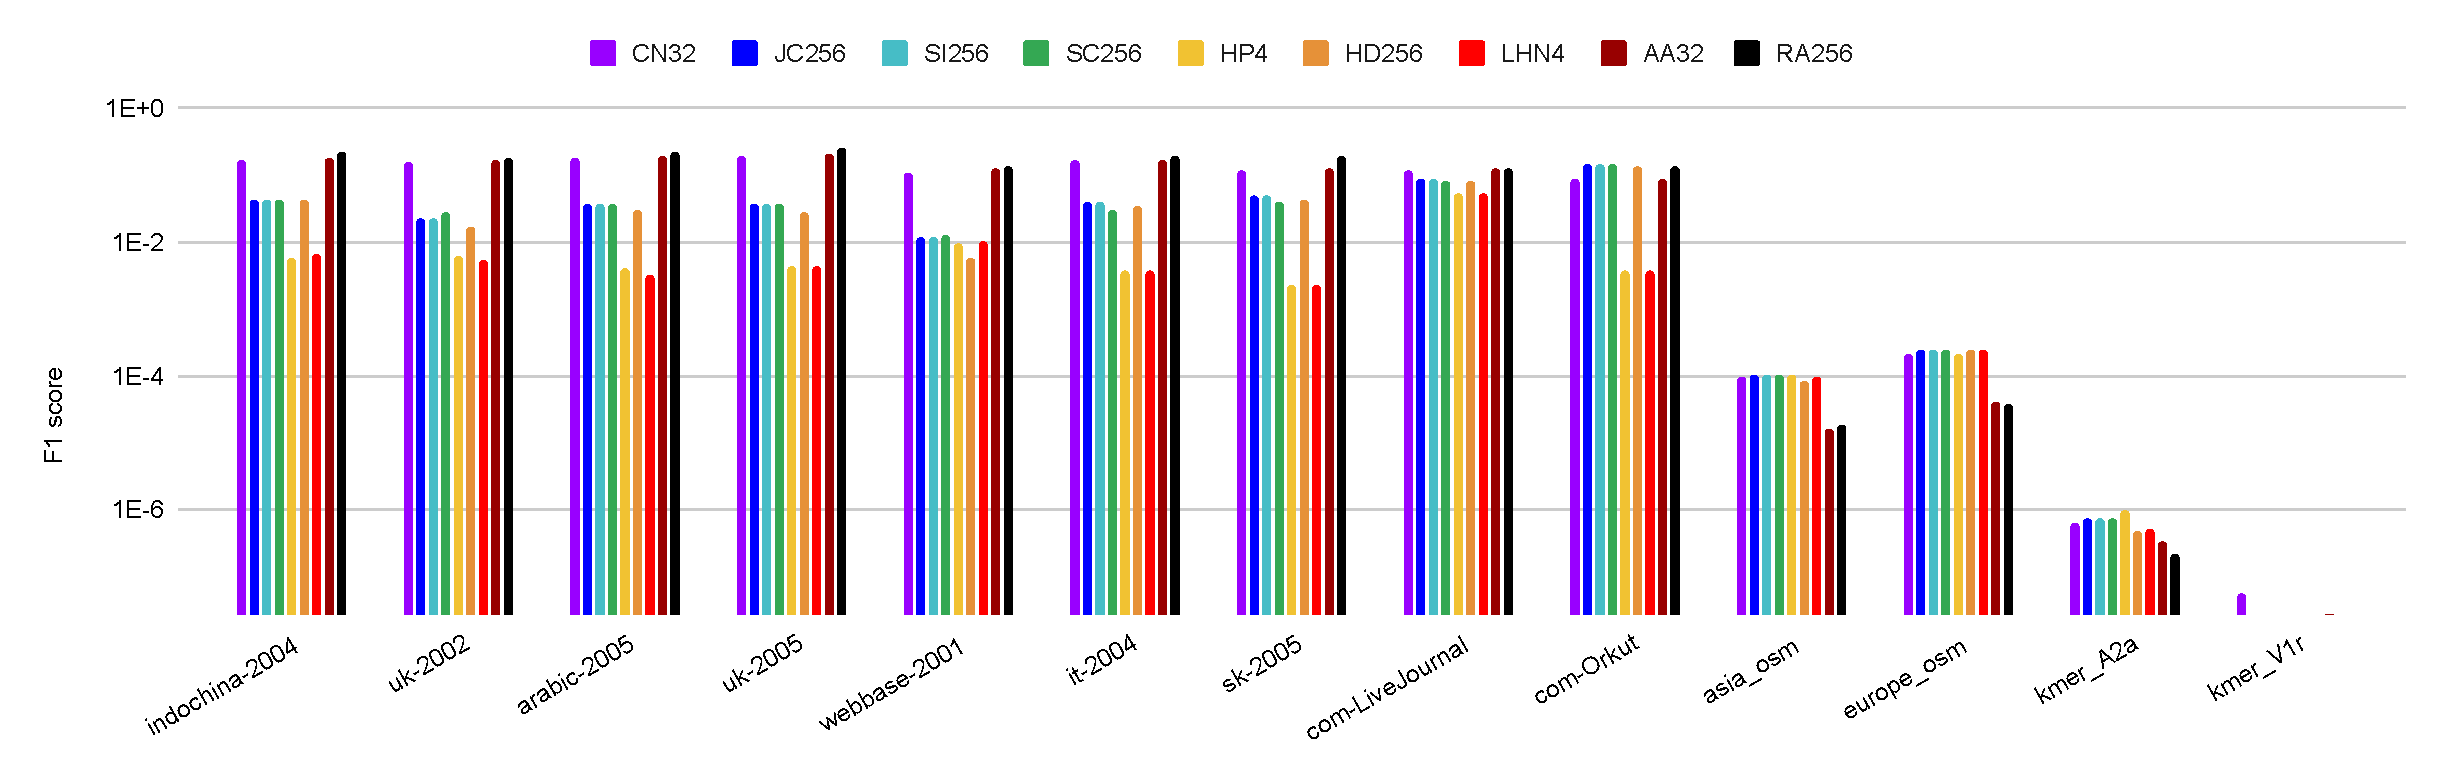
\includegraphics[width=0.98\linewidth]{out/pruned1-f1score.pdf}
  } \\[-2ex]
  \caption{TODO. Runtime in seconds (log-scale), and precision of predicted links, in percentage (log-scale), of the best neighborhood-based link prediction method (considering both the precision and runtime), on batch sizes of $10^{-4}|E|$ to $0.1|E|$ for each graph in the dataset. None of the methods succeed in predicting ground-truth links for \textit{kmer\_V1r}, and for \textit{asia\_osm} and \textit{kmer\_A2a} on batch sizes of $10^{-4}|E|$ to $10^{-3}|E|$, and thus their results are not shown. Note that the numerical suffix added to the acronym of each link prediction method indicates the hub limit $L_H$ parameter setting.}
  \label{fig:pruned1}
\end{figure*}
